%%%%%%%%%%%%%%%%%%%%%%%%%%%%%%%		CHAP 4		%%%%%%%%%%%%%%%%%%%%%%%%%%%%%%%

\chapter{Data Analysis procedures}
\label{cha:4}

 Interpreting the electronic signals produced by the detector is a mandatory step for event reconstruction %
 process.
 Energies, momenta, and directions of the involved particles must be established in order to determine %
 the detected physical interaction, whose study is the ultimate goal of the experiment.
 ANNIE's early stage data have been studied and analysis algorithms were developed and tested from scratch: %
 they are implemented in a purpose-built software, which studies the signals acquired from the water PMTs.
 The code's procedures relies on individual pulse analysis and it is largely focuses on the rejection of %
 background with respect to event signals.
 Some of these methods, illustrated, in this chapter could be employed into a more complete analysis %
 framework, valid even for the future phases of the experiment.

\section{Data selection}

 The Main DAQ is programmed to create a new \emph{Run} every time the Chain is stopped and restarted.
 Due to being an R\&D phase, the DAQ has been improved in various occasion during data taking, %
 hence the size and the number of post-processed files, that constitute the \emph{Runs}, are not constant.
 Nevertheless high statistics were achieved most of the time.
 The post-processed ROOT files (see section~ref) from the DAQ are used in the data analysis.
 The buffer retrieved from the VME boards is properly split for each trigger (hardware or software) signal, %
 in that each set of data consists of 80~$\mu$s worth of digitised signal.
 A single file holds 383 full buffers and this translates to 1532 triggers, or physically speaking to \np{122.560}~ms.

 Two distinctive couples of consecutive runs were selected as model data set, with the intention to %
 outline the best data analysis procedures.
 These are:
\begin{itemize}
  \item two runs with the beam off and a random trigger: these data are mostly \emph{cosmics};
  \item two runs with the \emph{beam} on, but with one PMT mounted on top of the NCV, in order to %
    observe the neutron capture.
\end{itemize}

 All the couples have been merged in single files after being scanned by the data analysis algorithm and %
 so treated as ones.
 Their quantitative features are shown in Tab.~\ref{tab:runs}.
 For the analysis's sake, the \emph{beam} and the \emph{cosmics} data set are the same, but for a different %
 photodetector.

\begin{table}
  \caption{Runs selected for data analysis. They are composed of different numbers of file, resulting in %
    diverse number of triggers. Total time is the number of triggers times 80~$\mu$s.
    The listed memory sizes refer to the post-processed files.}
  \label{tab:runs}
  \small
  \centering
  \begin{tabular}{crcrr}
    \toprule
    \textbf{Run type} & \textbf{N of files} & \textbf{N of Triggers} & \textbf{Total time} & \textbf{Data size} \\
    		 &      	&		& (ms)			& 	(MB)	            	\\
    \midrule	                                                                     
      Cosmics	 & 142	& \np{217544}	& \np{17403.520}	& \np{106130.447}	\\
      Beam	 & 164	& \np{251248}	& \np{20099.840}	& \np{122542.009}	\\
    \bottomrule
  \end{tabular}
\end{table}

\section{Individual pulse analysis}
%\textcolor{red}{Peak to valley suggests that a reflection occurs. Explain here or next?}

 The data analysis software scans all the post-processed time profile which the \emph{Run} consists of, %
 as the one shown in Fig.~\ref{fig:profile}, sorted by trigger and PMT number.
 Any peak above a certain voltage threshold, $V_T$, is selected and an enclosing time window %
 of a predefined length, $L$, is trimmed around it.
 A length of $L = 100$~samples was chosen, resulting in a \np{0.8}~$\mu$s long window.
 The position of the peak inside this window was set to 20\% of its length, i.e. the peak is always %
 set at \np{0.16}~$\mu$s from the beginning of the time window.
 These subsets of data are called \emph{pulses} and are collected in another ROOT file.
 The choice of window length and the peak position is the result of a compromise between speed of the code, %
 memory usage and loss of physical information.
 In fact, many pulses shows consecutive multiple peaks, as the one in Fig.~\ref{fig:pulse}, mainly given by %
 light reflections in the water tank.

 \begin{figure}
   \centering
   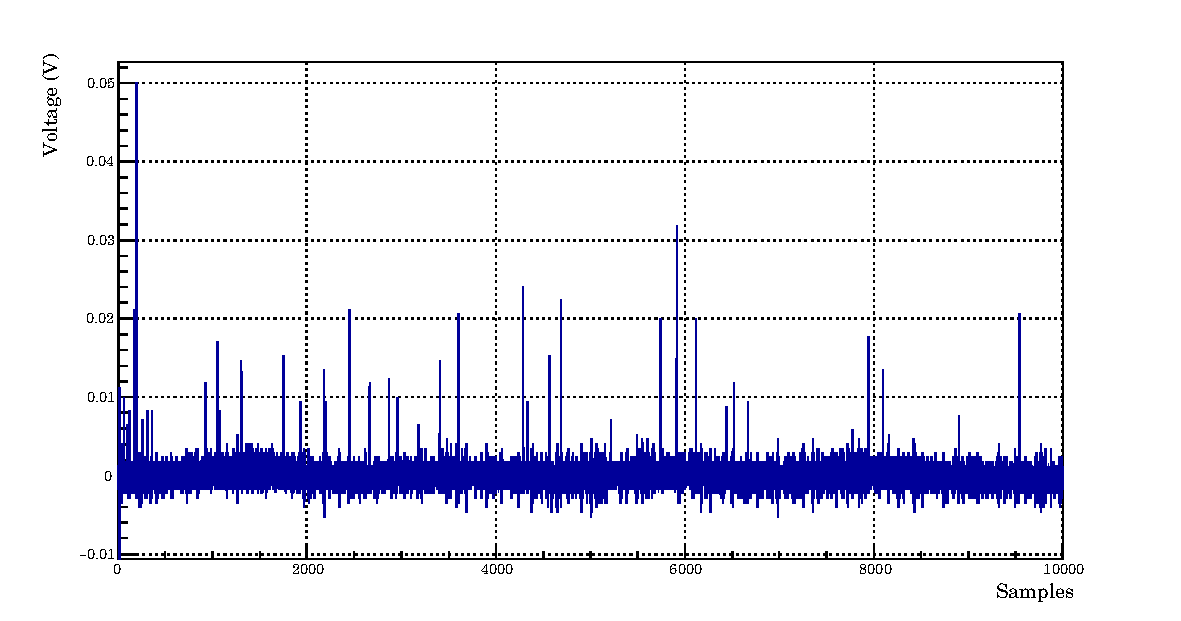
\includegraphics[scale=0.5]{pics/timeprofile.pdf}
   \caption{Time profile of a single trigger: the signals of the sixty PMTs are here overlaid.}
   \label{fig:profile}
 \end{figure}

 \begin{figure}
   \centering
   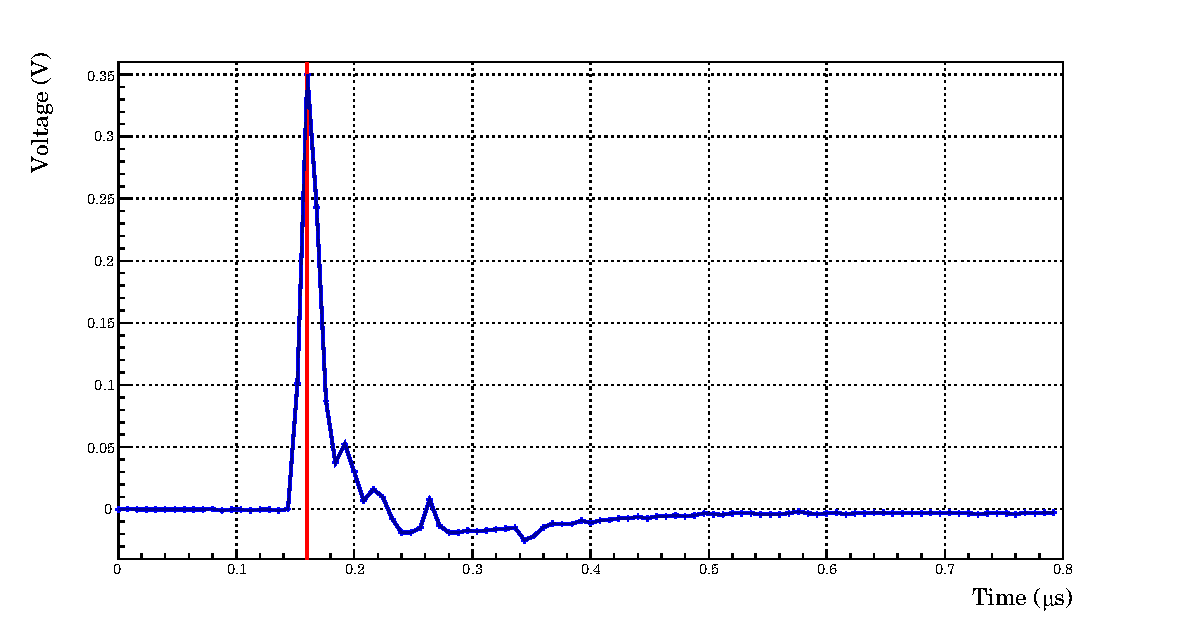
\includegraphics[scale=0.5]{pics/pulse.pdf}
   \caption{Time profile of a single pulse. The red line marks the 20\,\% of the window's length, at $\np{0.16}~\mu$s. %
     The first peak and the second peak are about forty nanoseconds apart, which is the time needed for the light to %
   travel back and forth inside the tank (see section~ref).}
   \label{fig:pulse}
 \end{figure}

 Each pulse is individually analysed and processed by a routine of algorithms.
 As a result, a set of values is gathered from every pulse, in addition to Veto and MRD coincidences.
 These quantities, outlined in Fig.~\ref{fig:pulseana}, are useful for following analysis and they are labelled:

\begin{description}
  \item[\bfseries Baseline]: it is the average of first 10 points of the pulse; %
    this value is then subtracted from the whole array.
  \item[\bfseries Height]: it is the height of the peak (maximum) with respect to the zero.
  \item[\bfseries Peak to valley]: it is the time distance from the peak to the valley (minimum).
  \item[\bfseries Start]: it is the position of the 25\% of the rising edge of the pulse, estimated with %
    precision using cubic interpolation
  \item[\bfseries Width]: it is the time that spans from Start to the 5\% of the falling edge %
    of the pulse (End), calculated using the same algorithm employed for Time.
  \item[\bfseries Charge]: it is the sum of the 5 points around peak, weighted with the bin width.
  \item[\bfseries Energy]: it is the signal integral form the Start to the End.
  \item[\bfseries Area]: it is the area of the modulus of the pulse.
  \item[\bfseries Time of flight]: is the time difference between the Start and RWM signal.
  \item[\bfseries Previous]: is the time difference between the Start and the Start of the previous pulse, %
    if from the same PMT.
\end{description}

\begin{figure}
  \centering
  \def\svgwidth{0.47\textwidth}
  \subfloat[From left to right: in green the \emph{BaseLine}, in orange the \emph{Peak Height}, %
  in purple the \emph{Width}, and in light blue the \emph{Peak to Valley} time distance.]%
  {\import{pics/}{timepoints.pdf_tex}} \qquad
  \def\svgwidth{0.47\textwidth}
  \subfloat[From left to right: in pink the \emph{Charge}, in blue the \emph{Energy}, and in gold the \emph{Area}. %
  These three integrals cross over each other in the purple region.]%
  {\import{pics/}{areapoints.pdf_tex}}
  \caption{Illustration of the pulse analysis values. The \emph{25\,\%} and \emph{5\,\% peak height} marks, %
  which define the \emph{Start} and \emph{End} of the signal, are common to both diagrams. The dashed lines represent %
  the cubic interpolations.}
  \label{fig:pulseana}
\end{figure}

 Being a water Cherenkov detector, the event reconstruction in ANNIE relies on time and energy of the signals %
 and for this fact these two quantities must be measured precisely.
 The time position of the pulses, or \emph{Start}, is thus determined with high precision thanks to data %
 interpolation\footnote{The algorithm looks for four points around the threshold (25\,\% for the \emph{Start} %
   or 5\,\% for the \emph{End}), which are used to define a cubic function. Using Newton's method, the correct %
   time position is found.}, within the time resolution of the ADCs.
 In Fig.~a of~\ref{fig:spectrum} the spectrum of the \emph{Starts} of a beam run is plotted: the frequency boost %
 with respect to the background suggests that the beam occurs ten microseconds after the beginning of the data %
 acquisition.
 The distinctive trait of the neutron capture by gadolinium is a delayed signal, detected 20-30~$\mu$s.
 Therefore studying the relative time distance between pulses is fundamental, particularly in the ANNIE experiment.
 The \emph{Previous} entry has the potential to accomodate this neccessity and reveal other interesting features.
 For instance, in Fig.~b of~\ref{fig:spectrum} \emph{Start} is plotted against \emph{Previous}.

 \begin{figure}
   \centering
   \subfloat[The beam is clearly visible at the beginning of the 80~$\mu$s buffer; the second half is basically free of %
   beam related events. ]{\includegraphics[width=0.47\textwidth]{pics/timefreq.pdf}}\,
   \subfloat[\emph{Start} is plotted against \emph{Previous}; both axes are in $\mu$s.
   The beam pulses are split into two groups: the pulses in the red ellipse are independent of their previous pulse, %
   while a correlation is visible in the set of the blue ellipse.]%
   {\includegraphics[width=0.47\textwidth]{pics/startvsnext.png}}
  \caption{Time distribution of the pulses of a beam run.}
   \label{fig:spectrum}
 \end{figure}

 On the other hand, estabilishing the signals' energy is more complicated, since the PMTs have not been calibrated yet.
 However, the photodetectors are set with the same gain, therefore an evaluation of the pulse integral is a good %
 indicator of the total charge deposited on each PMT.
 Three different methods to estimate the area enclosed in a pulse integral have been implemented.
 The names \emph{Charge}, \emph{Energy}, and \emph{Area} were only chosen in order to distinguish them from each other.
 As suggested from Fig.~\ref{fig:pulse}, there is a partial superimposition of the three: they show indeed %
 interesting correlation patterns, reported in Fig.~\ref{fig:integral}.

\begin{figure}
  \centering
  \subfloat[The \emph{Charge} is plotted against the \emph{Energy}]%
  {\includegraphics[width=0.47\textwidth]{pics/chargevsenergy.png}}\,
  \subfloat[The \emph{Area} is plotted against the \emph{Energy}]%
  {\includegraphics[width=0.47\textwidth]{pics/areavsenergy.png}}\\
  \subfloat[The \emph{Area} is plotted against the \emph{Charge}]%
  {\includegraphics[width=0.47\textwidth]{pics/areavscharge.png}}
  \subfloat[The spectrum of \emph{Width}.]%
  {\includegraphics[width=0.47\textwidth]{pics/width.pdf}}
  \caption{Correlation plots among the three integral quantities. The red lines isolate areas with different %
  correlation, likely due to different widths of the pulses.}
  \label{fig:integral}
\end{figure}

 For every Trigger, the time distribution of the peaks is studied, as well as the time coincidences %
 between the PMTs signals: a time allowance of $\np{0,8}~\mu$s is considered to count of pulses happening %
 simultaneously; this easily translates to the number of PMTs fired at the same time.
 When the latter exceeds a defined threshold, $N_{PMT}$, then an \emph{Event} is appointed and its precise time %
 position is afterwards estimated by a weighted average of the adjacent coincidences.
% The time tolerancy is high enough to include most of the in a way that all the light from the interaction is counted
 The multiplicity of an Event is a good indicator of the nature of the detected interaction.
 As discussed in section~ref, a cosmic muon, likely coming from above, would project the Cherenkov radiation on the %
 bottom of the tank, thus lighting the majority of the water PMTs.
 On the other hand, a muon arisen from the interaction of a beam neutrino with a nucleon would emit gammas %
 along the beam direction: only a portion of the light cone could be captured, hence the PMTs would be partially %
 triggered.
 Even natural radioactivity, from radionuclide in the glass of the phototubes, can be detected, although %
 these events have lower multiplicity and are readily filtered by a proper threshold of $N_{PMT}$.
 An high-multiplicity event is exemplified in Fig.~\ref{fig:event}.

  \begin{figure}
   \centering
   \subfloat[The red line marks the weighted average of the coincidences, which is $\np{34.51}~\mu$s in this example.]%
   {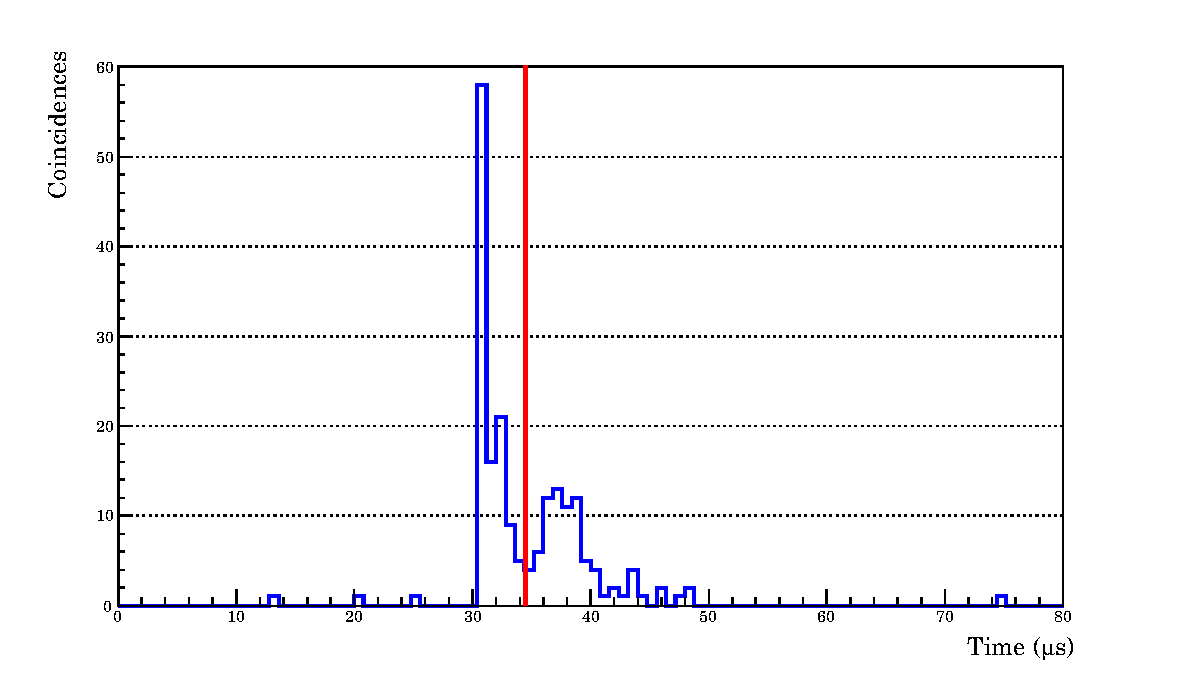
\includegraphics[width=0.47\textwidth]{pics/coincidences.pdf}}\,
   \subfloat[The coloured lines mark the five time window for noise rejection, $\Delta_T$ in $\mu$s, %
   listed in Tab.~\ref{tab:thr_var}.]{\includegraphics[width=0.47\textwidth]{pics/rejection.pdf}}
   \caption{Both plots show the same histogram, filled with the \emph{Start} time of each pulse belonging to %
   the same trigger. An high multiplicity event is found near $\np{31}~{\mu}$s.
   In this particular case, the time distribution of the signals is quite long: %
   the light in the tank lasts for about twenty microseconds.}
   \label{fig:event}
 \end{figure}

 Not every pulse in a trigger belongs to an event.
 For instance, in Fig.~\ref{fig:event} there are at least four pulses outside from the main pulse cluster.
 These might be likely generated by noise sources and therefore they are useless in view of the event %
 reconstruction.
 In order to discriminate the pulses, an arbitrary time interval, whose radius is $\Delta_T$, is defined around %
 the Event time position.
 Every pulse that falls within this window is designated as a \emph{signal}; otherwise it is \emph{noise}.

\section{Signal and noise discrimination}

 Discriminating signal from background is a step of utmost importance for data analysis.
 Being a first stage study, the algorithm only relies on $V_T$, $N_{PMT}$, and $\Delta_T$, %
 in order to distinguish event pulses from noise ones.
 It is necessary, even for future analysis framework, to determine the best combination of the three parameters.
 To achieve that, these have been varied and the data have been analysed multiple times.
 Twelve combination were chosen and they are listed in Tab.~\ref{tab:thr_var}.
 The variation of the voltage threshold affects the total number of pulses, because any peak below $V_T$ is %
 neglected.
 The five values employed are all well above the electronic noise, which is of the order of the millivolt.

 The ratio between \emph{signals} and \emph{noises} is rather governed by the other two parameters, %
 the number of PMTs fired and the rejection time window.
 Respectively four and five values were picked for these parameters.
 The increase of $N_{PMT}$ restricts the number of \emph{events}, as suggested by Fig.~\ref{fig:npmt} where the %
 multeplicity of the events is plotted.
 This values is indeed closely related to the number of PMTs hit in an interaction.
 The rise in the frequency, near the end of the x-axis, is likely due to high multeplicity cosmic muon events.
 The time allowance of the \emph{event} definition was also studied, varying the $\Delta_T$ parameter.
 Understanding the relevance of belated photons, possibily given by reflection inside the tank, is decisive for %
 developing a correct analysis framework.
 The selected intervals are illustrated in Fig.~b of~\ref{fig:event}.

 \begin{figure}
   \centering
   \includegraphics[width=0.5\textwidth]{pics/pmt.pdf}
   \caption{Frequency of the number of PMTs hit in an event.}
   \label{fig:npmt}
 \end{figure}

% \begin{wraptable}{r}{0.5\textwidth}
 \begin{table}
  \caption{The combination of the employed thresholds.
    The first one, in bold letters, is common to each subset.}
  \label{tab:thr_var}
  \centering
  \small
  \begin{tabular}{lccc}
    \toprule
    \textbf{Label}	& $V_T$		& $N_{PMT}$		& $\Delta_T$	\\
    	&	(V)	 		& 			& ($\mathrm{\mu}$s)			\\
    \midrule
    $C$	&	\textbf{\np{0.02}}	& \textbf{10}		& \textbf{\np{4.0}}		\\
    \midrule
    $V_{00}$	&	    \np{0.005}		& 10			& \np{4.0}			\\
    $V_{01}$	&	\np{0.01}		& 10			& \np{4.0}			\\
    $V_{05}$	&	\np{0.05}		& 10			& \np{4.0}			\\
    $V_{10}$	&	\np{0.10}		& 10			& \np{4.0}			\\
    \midrule
    $N_{15}$	&	\np{0.02}		& 15			& \np{4.0}			\\
    $N_{30}$	&	\np{0.02}		& 30			& \np{4.0}			\\
    $N_{50}$	&	\np{0.02}		& 50			& \np{4.0}			\\
    \midrule
    $\Delta_{50}$	& \np{0.02}		& 10			& \np{5.0}			\\
    $\Delta_{30}$	& \np{0.02}		& 10			& \np{3.0}			\\
    $\Delta_{20}$	& \np{0.02}		& 10			& \np{2.0}			\\
    $\Delta_{10}$	& \np{0.02}		& 10			& \np{1.0}			\\
    \bottomrule
  \end{tabular}
 \end{table}
 %\end{wraptable}

 The processed data sets present therefore different number of pulses and different proportion between signals %
 and noises.
 Every collection of processed data is then studied a posteriori and tested with diversified methods. 
